\begin{figure}[t]
    \centering
    \begin{subfigure}{0.49\linewidth}
        \centering
        \resizebox{1\linewidth}{!}{% This file was created by matlab2tikz.
%
%The latest updates can be retrieved from
%  http://www.mathworks.com/matlabcentral/fileexchange/22022-matlab2tikz-matlab2tikz
%where you can also make suggestions and rate matlab2tikz.
%
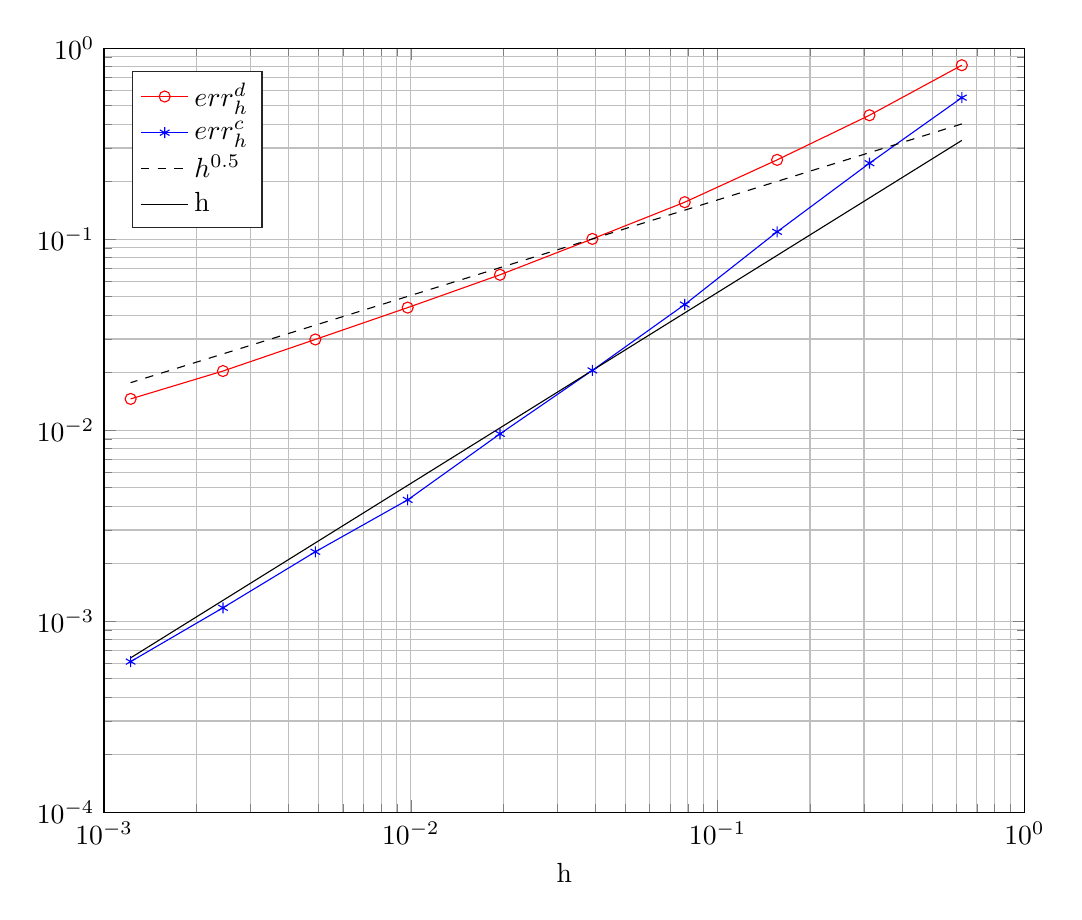
\begin{tikzpicture}

\begin{axis}[%
width=4.602in,
height=3.82in,
at={(0.772in,0.516in)},
scale only axis,
xmode=log,
xmin=0.001,
xmax=1,
xminorticks=true,
xlabel={h},
xmajorgrids,
xminorgrids,
ymode=log,
ymin=0.0001,
ymax=1,
yminorticks=true,
ymajorgrids,
yminorgrids,
axis background/.style={fill=white},
legend style={at={(0.03,0.97)},anchor=north west,legend cell align=left,align=left,draw=white!15!black}
]
\addplot [color=red,solid,mark=o,mark options={solid}]
  table[row sep=crcr]{%
0.625	0.814121166527388\\
0.3125	0.445308666527388\\
0.15625	0.260074291527388\\
0.078125	0.156160229027388\\
0.0390625	0.100300854027388\\
0.01953125	0.0650840571523877\\
0.009765625	0.0438213618398876\\
0.0048828125	0.0298496821523877\\
0.00244140625	0.0203989985586377\\
0.001220703125	0.0145757563711377\\
};
\addlegendentry{$\text{err}_\text{h}^\text{d}$};

\addplot [color=blue,solid,mark=asterisk,mark options={solid}]
  table[row sep=crcr]{%
0.625	0.550496166527388\\
0.3125	0.249839916527388\\
0.15625	0.109277416527388\\
0.078125	0.0454727290273877\\
0.0390625	0.0205547602773877\\
0.01953125	0.00956257277738766\\
0.009765625	0.00431550246488765\\
0.0048828125	0.00230768996488766\\
0.00244140625	0.00117487746488766\\
0.001220703125	0.000614086449262655\\
};
\addlegendentry{$\text{err}_\text{h}^\text{c}$};

\addplot [color=black,dashed]
  table[row sep=crcr]{%
0.625	0.401203416109551\\
0.3125	0.283693656166271\\
0.15625	0.200601708054775\\
0.078125	0.141846828083136\\
0.0390625	0.100300854027388\\
0.01953125	0.0709234140415679\\
0.009765625	0.0501504270136938\\
0.0048828125	0.0354617070207839\\
0.00244140625	0.0250752135068469\\
0.001220703125	0.017730853510392\\
};
\addlegendentry{$\text{h}^{\text{0.5}}$};

\addplot [color=black,solid]
  table[row sep=crcr]{%
0.625	0.328876164438203\\
0.3125	0.164438082219101\\
0.15625	0.0822190411095506\\
0.078125	0.0411095205547753\\
0.0390625	0.0205547602773877\\
0.01953125	0.0102773801386938\\
0.009765625	0.00513869006934691\\
0.0048828125	0.00256934503467346\\
0.00244140625	0.00128467251733673\\
0.001220703125	0.000642336258668364\\
};
\addlegendentry{h};

\end{axis}
\end{tikzpicture}% }  
        \caption{Killing boundary in $x = 1$}
        \label{fig:KillOneD}
    \end{subfigure}
    \begin{subfigure}{0.49\linewidth}
        \centering
        \resizebox{1\linewidth}{!}{% This file was created by matlab2tikz.
%
%The latest updates can be retrieved from
%  http://www.mathworks.com/matlabcentral/fileexchange/22022-matlab2tikz-matlab2tikz
%where you can also make suggestions and rate matlab2tikz.
%
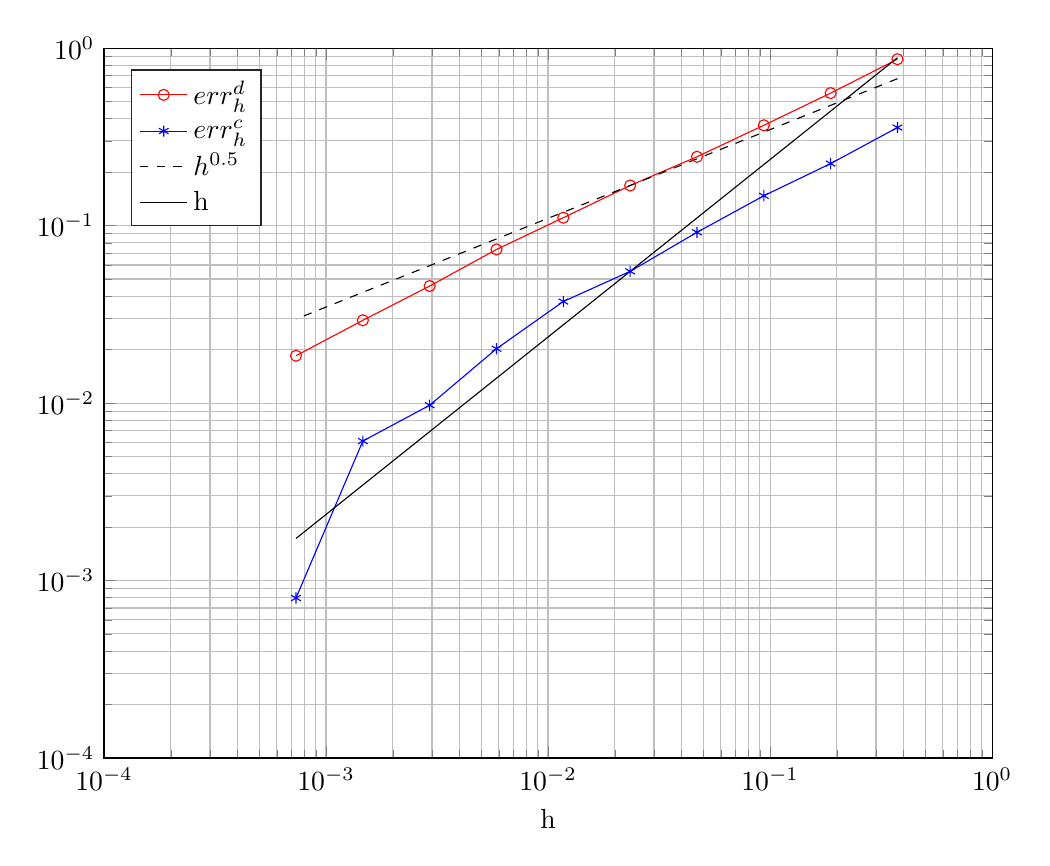
\begin{tikzpicture}

\begin{axis}[%
width=4.44in,
height=3.549in,
at={(0.745in,0.479in)},
scale only axis,
xmode=log,
xmin=0.0001,
xmax=1,
xminorticks=true,
xlabel={h},
xmajorgrids,
xminorgrids,
ymode=log,
ymin=0.0001,
ymax=1,
yminorticks=true,
ymajorgrids,
yminorgrids,
axis background/.style={fill=white},
legend style={at={(0.03,0.97)},anchor=north west,legend cell align=left,align=left,draw=white!15!black}
]
\addplot [color=red,solid,mark=o,mark options={solid}]
  table[row sep=crcr]{%
0.375	0.866448920874179\\
0.1875	0.558236420874179\\
0.09375	0.367633295874179\\
0.046875	0.244380170874179\\
0.0234375	0.168257514624179\\
0.01171875	0.110787592749179\\
0.005859375	0.0734094677491791\\
0.0029296875	0.0456410107179291\\
0.00146484375	0.0292624462648041\\
0.000732421875	0.0184820751710541\\
};
\addlegendentry{$\text{err}_\text{h}^\text{d}$};

\addplot [color=blue,solid,mark=asterisk,mark options={solid}]
  table[row sep=crcr]{%
0.375	0.357161420874179\\
0.1875	0.223680170874179\\
0.09375	0.147283295874179\\
0.046875	0.0916567333741791\\
0.0234375	0.0552278271241791\\
0.01171875	0.0373567333741791\\
0.005859375	0.0202379833741791\\
0.0029296875	0.0097233349366791\\
0.00146484375	0.00610927243667908\\
0.000732421875	0.000796943335116596\\
};
\addlegendentry{$\text{err}_\text{h}^\text{c}$};

\addplot [color=black,dashed]
  table[row sep=crcr]{%
0.375	0.673030058496717\\
0.1875	0.475904118305407\\
0.09375	0.336515029248358\\
0.046875	0.237952059152704\\
0.0234375	0.168257514624179\\
0.01171875	0.118976029576352\\
0.005859375	0.0841287573120896\\
0.0029296875	0.0594880147881759\\
0.00146484375	0.0420643786560448\\
0.000732421875	0.0297440073940879\\
};
\addlegendentry{$\text{h}^{\text{0.5}}$};

\addplot [color=black,solid]
  table[row sep=crcr]{%
0.375	0.883645233986866\\
0.1875	0.441822616993433\\
0.09375	0.220911308496716\\
0.046875	0.110455654248358\\
0.0234375	0.0552278271241791\\
0.01171875	0.0276139135620896\\
0.005859375	0.0138069567810448\\
0.0029296875	0.00690347839052239\\
0.00146484375	0.00345173919526119\\
0.000732421875	0.0017258695976306\\
};
\addlegendentry{h};

\end{axis}
\end{tikzpicture}% }  
        \caption{Reflecting boundary in $x = 1$}
        \label{fig:ReflectOneD}
    \end{subfigure}    
    \caption{Approximation of $\tau$. Orders of convergence for DEM and CEM in the one-dimensional case.}
    \label{fig:OrdersOneD}
\end{figure}

\begin{figure}[t]
    \centering
    \begin{subfigure}{0.49\linewidth}
        \centering
        \resizebox{1\linewidth}{!}{% This file was created by matlab2tikz.
%
%The latest updates can be retrieved from
%  http://www.mathworks.com/matlabcentral/fileexchange/22022-matlab2tikz-matlab2tikz
%where you can also make suggestions and rate matlab2tikz.
%
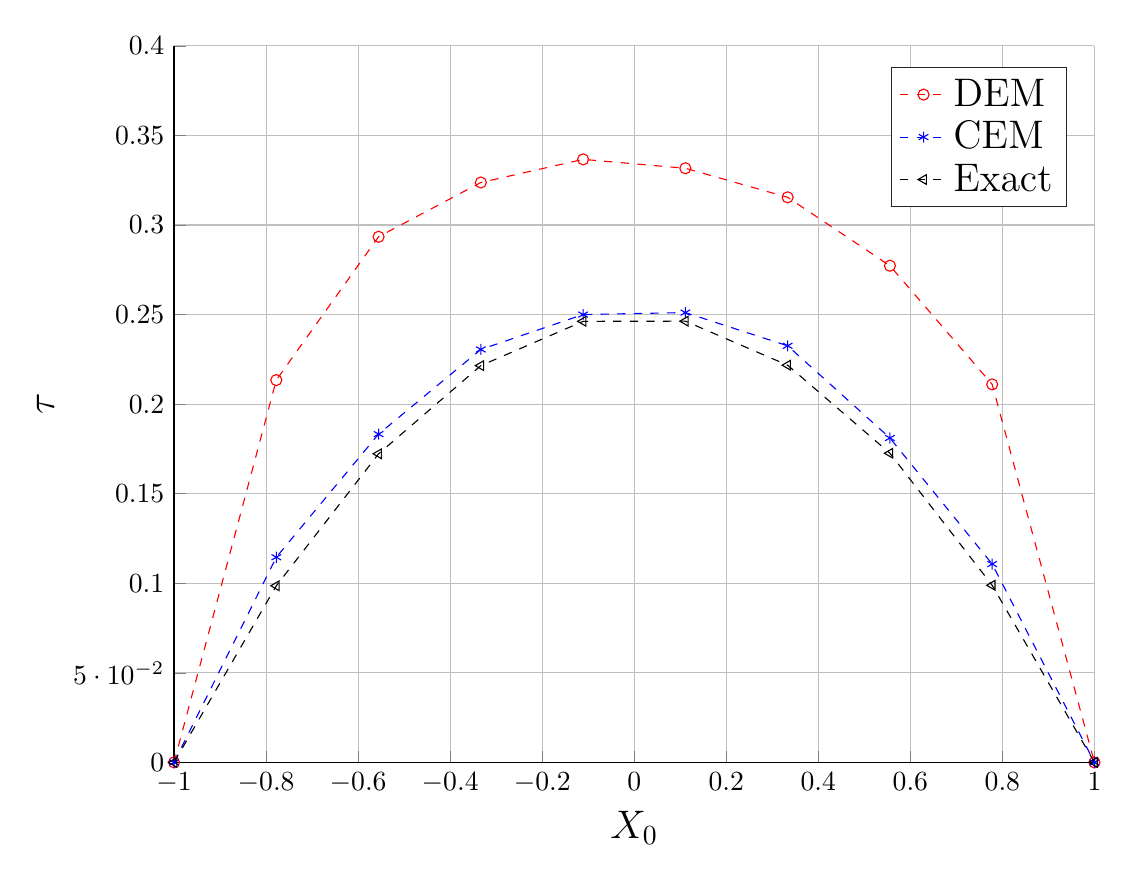
\begin{tikzpicture}

\begin{axis}[%
width=4.602in,
height=3.583in,
at={(0.772in,0.484in)},
scale only axis,
xmin=-1,
xmax=1,
xlabel={$X_0$},
xlabel style = {font = \Large},
xmajorgrids,
ymin=0,
ymax=0.4,
ylabel={$\tau$},
ylabel style = {font = \Large},
ymajorgrids,
axis background/.style={fill=white},
axis x line*=bottom,
axis y line*=left,
legend pos = north east,
legend style={legend cell align=left,align=left,draw=white!15!black,font=\Large}
]
\addplot [color=red,dashed,mark=o,mark options={solid}]
  table[row sep=crcr]{%
-1	0\\
-0.777777777777778	0.213421875\\
-0.555555555555556	0.2934140625\\
-0.333333333333333	0.3236953125\\
-0.111111111111111	0.336609375\\
0.111111111111111	0.331640625\\
0.333333333333333	0.315421875\\
0.555555555555556	0.2772421875\\
0.777777777777778	0.2110078125\\
1	0\\
};
\addlegendentry{DEM};

\addplot [color=blue,dashed,mark=asterisk,mark options={solid}]
  table[row sep=crcr]{%
-1	0\\
-0.777777777777778	0.114515625\\
-0.555555555555556	0.1832578125\\
-0.333333333333333	0.2305078125\\
-0.111111111111111	0.249984375\\
0.111111111111111	0.2510859375\\
0.333333333333333	0.232546875\\
0.555555555555556	0.181078125\\
0.777777777777778	0.11071875\\
1	0\\
};
\addlegendentry{CEM};

\addplot [color=black,dashed,mark=triangle,mark options={solid,rotate=90}]
  table[row sep=crcr]{%
-1	0\\
-0.777777777777778	0.0986011931395157\\
-0.555555555555556	0.172254291984329\\
-0.333333333333333	0.221472162307402\\
-0.111111111111111	0.246204174763737\\
0.111111111111111	0.2462957329545\\
0.333333333333333	0.221719125026098\\
0.555555555555556	0.172574095814315\\
0.777777777777778	0.0988572350577004\\
1	0\\
};
\addlegendentry{Exact};

\end{axis}
\end{tikzpicture}%
 }  
        \caption{Killing boundary in $x = 1$}
        \label{fig:ApproxOneD}
    \end{subfigure}
    \begin{subfigure}{0.49\linewidth}
        \centering
        \resizebox{1\linewidth}{!}{% This file was created by matlab2tikz.
%
%The latest updates can be retrieved from
%  http://www.mathworks.com/matlabcentral/fileexchange/22022-matlab2tikz-matlab2tikz
%where you can also make suggestions and rate matlab2tikz.
%
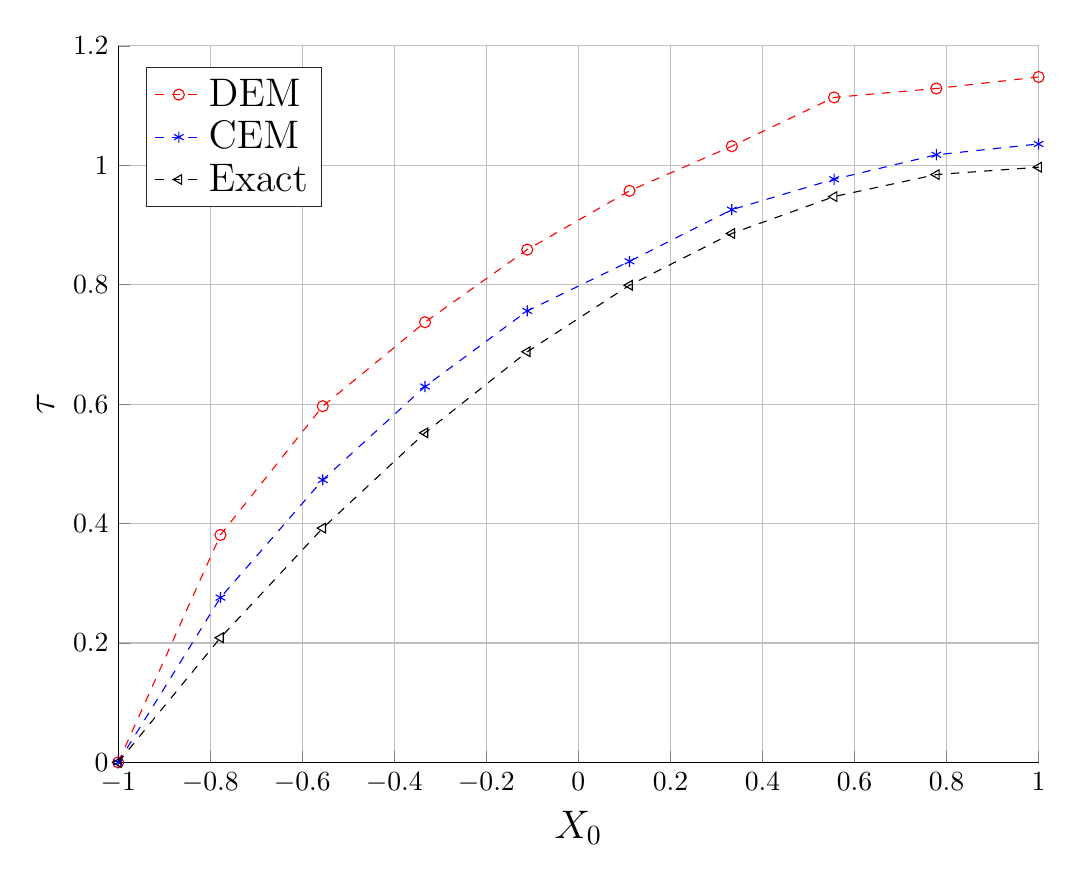
\begin{tikzpicture}

\begin{axis}[%
width=4.602in,
height=3.583in,
at={(0.772in,0.484in)},
scale only axis,
xmin=-1,
xmax=1,
xlabel={$X_0$},
xlabel style={font=\Large},
xmajorgrids,
ymin=0,
ymax=1.2,
ylabel={$\tau$},
ylabel style={font=\Large},
ymajorgrids,
axis background/.style={fill=white},
axis x line*=bottom,
axis y line*=left,
legend style={at={(0.03,0.97)},anchor=north west,legend cell align=left,align=left,draw=white!15!black,font=\Large}
]
\addplot [color=red,dashed,mark=o,mark options={solid}]
  table[row sep=crcr]{%
-1	0\\
-0.777777777777778	0.3809765625\\
-0.555555555555556	0.5964609375\\
-0.333333333333333	0.73715625\\
-0.111111111111111	0.8587265625\\
0.111111111111111	0.9571171875\\
0.333333333333333	1.031859375\\
0.555555555555556	1.113609375\\
0.777777777777778	1.1285390625\\
1	1.1478046875\\
};
\addlegendentry{DEM};

\addplot [color=blue,dashed,mark=asterisk,mark options={solid}]
  table[row sep=crcr]{%
-1	0\\
-0.777777777777778	0.275953125\\
-0.555555555555556	0.4729921875\\
-0.333333333333333	0.629484375\\
-0.111111111111111	0.7560703125\\
0.111111111111111	0.8390625\\
0.333333333333333	0.9255703125\\
0.555555555555556	0.976546875\\
0.777777777777778	1.017515625\\
1	1.035609375\\
};
\addlegendentry{CEM};

\addplot [color=black,dashed,mark=triangle,mark options={solid,rotate=90}]
  table[row sep=crcr]{%
-1	0\\
-0.777777777777778	0.208777054487475\\
-0.555555555555556	0.392333503315235\\
-0.333333333333333	0.551939853868488\\
-0.111111111111111	0.687661056545228\\
0.111111111111111	0.79906851214989\\
0.333333333333333	0.885727939207175\\
0.555555555555556	0.947463001823471\\
0.777777777777778	0.984384604394486\\
1	0.996687130893952\\
};
\addlegendentry{Exact};

\end{axis}
\end{tikzpicture}%
 }  
        \caption{Reflecting boundary in $x = 1$}
        \label{fig:ApproxOneD}
    \end{subfigure}    
    \caption{Approximation of $\tau$ as a function of the initial value $X_0$.}
    \label{fig:ApproxOneD}
\end{figure}
